\documentclass{article}
\usepackage{graphicx}
\usepackage{subcaption}
\usepackage{caption}
\usepackage{subcaption}
\usepackage[utf8]{inputenc}
\usepackage{relsize,makeidx,color,setspace,amsmath,amsfonts,amssymb}
\title{FYS3150 - Project 4}
\author{Synne Skinnes Hansen}
\date{November 2017}
\begin{document}
\maketitle
\section*{Abstract}

\section*{Introduction}
The aim of this project is to study phase transitions in magnetic systems using the Ising model in two dimensions. A phase transition is marked by abrupt macroscopic changes, in our model we will have a spontaneous magnetization equal to zero below a critical temperature.
The model will be solved numerically by using the Metropolis algorithm. It is possible to find an analytical expression for a simple lattices with few states, but when the lattice gets bigger this becomes impossible. 
Anyway, to solve this we will start of by finding the analytic expressions for different thermodynamic quantities using a simple 2x2 lattice. This will be used to determine the optimal number of Monte Carlo cycles needed to achieve a good agreement later. 
Since its impossible to solve the Ising model analytical for higher dimensions we need to solve it numerically. 
To solve the model analytically 
Then we increase the lattice and study how many cycles needed in order to reach equilibrium state. We do this by looking at the time corresponding to the number of cycles.
Finally we will study the behavior of the Ising model close to the critical temperature by looking at larger lattices. These simulations will then be used to extract the critical temperature. 

\section*{Methods}
The model we will use in our studies of phase transitions at finite temperature for magnetic systems, is the Ising model. This model consists of discrete variables that represents magnetic dipole moments of atomic spins in two states, pointing up or down. The spins will are arranged in a lattice, allowing each spin to interact with its neighbors. We will also use periodic boundary conditions . 
In one and two dimensions, for small lattices, it is easy to find an analytic solution to several expectation values. For higher lattices we will use the Metropolis algorithm to solve the problem numerically. 
\subsection*{Canonical Ensemble}
In mathematical physics an ensemble is a probability distribution for the state of a system. In this project we will use the canonical ensemble for our calculations. 
In order to find the analytical expressions for the expectation values we need a probability distribution.The Bolzmann distribution gives us the probability of particles in a system over various possible states for a given temperature. It is given by 
$$P_i(\beta) = \frac{e^{-\beta E_i}}{Z} $$
with $\beta = 1/k_B T$. $k_B$ is the Bolzmann constant, $E_i$ is the energy of a microstate $i$, while $Z$ is the partion function defined as 
$$Z = \sum_{i=1}^M e^{-\beta E_i}$$
where the sum extends over all microstates M. This distribution shows us that states with lower energy always will have a higher possibility of being occupied than the states with higher energy. 
\subsubsection*{Thermodynamic quantities}
For later studies of phase transistions we want to look at different thermodynamic quantites. 
Energy and mean magnetization are expectation values since we allow them to be exchanged with the surroundings. They can be calculated by the probability distribution, given by:
$$<E> = \frac{1}{Z}\sum_{i=1}^M E_ie^{-\beta E_i}$$ 
$$<M> = \frac{1}{Z}\sum_{i=1}^M M_ie^{-\beta E_i} $$
where $M_i$ is the magnetization in a given state $i$. 
The corresponding variance is defined as
$$\sigma^2_E = <E^2> - <E>^2 $$
The variance divided by the latter quantity $kT^2$ gives us the specific heat: 
$$C_V = \frac{1}{k_B T}(<E^2> - <E>^2)$$
Using the same prescription for the magnetization, we get the susceptibility: 
$$\chi = \frac{1}{k_B T}(<M^2> - <M>^2)$$
\subsection*{The Ising Model}
\subsubsection*{Energy}
The energy of the Ising model is expressed as 
$$E = -J\sum_{<kl>}^Ns_k s_l $$
when we have no magnetic field. We have $s_k = \pm$, $N$ is the total number of spins, $J$ is a constant expressing the strength of the interacting between neighboring and $<kl>$ indicates the sum over the nearest neighbours only. 
This leads to spontaneous magnetization at low temperatures.
\subsubsection*{Phase transitions}
This model undergoes a phase transition of second order. This means that below a critical temperature $T_C$ the model exhibits a spontaneous magnetization with $<M> != 0$. 
For the ising model we can characterise the behaviour of many physical quantities near $T_C$. 
The correlation length is such an important quantity and is expected to be of the order of the lattice spacing $T>>T_C$. When $T$ approches $T_C$, the spins becomes more and more correlated. Then the correlation length $\xi$ increases as we get closer to the critical temperature. The divergent behavior of $\xi$ near $T_C$ is 
\begin{equation}
  \xi(T) \sim \left|T_C-T\right|^{-\nu}.
  \label{eq:xi}
\end{equation}
A second-order phase transition is characterized by a correlation length which spans the whole system. In this project we are always limited to a finite lattice and $\ri$ will be proportional with the size of the lattice at the critical point. Finite size scaling relations relate the behavior at finite lattices with the results for infinitely large lattice. The critical temperature scales then as: 
\begin{equation}
 T_C(L)-T_C(L=\infty) = aL^{-1/\nu},
 \label{eq:tc}
\end{equation}
where $a$ and $\nu$ is constants. When $T = T_C$ we obtain the following: 
\begin{equation*}
  \langle {\cal M}(T) \rangle \sim \left(T-T_C\right)^{\beta}
  \rightarrow L^{-\beta/\nu},
  \label{eq:scale1}
\end{equation*}
\begin{equation*}
  C_V(T) \sim \left|T_C-T\right|^{-\gamma} \rightarrow L^{\alpha/\nu},
  \label{eq:scale2}
\end{equation*}
\begin{equation*}
  \chi(T) \sim \left|T_C-T\right|^{-\alpha} \rightarrow L^{\gamma/\nu}.
  \label{eq:scale3}
\end{equation*}

\subsection*{Metropolis algorithm}
The main numerical method we will use to solve the problem is The Metropolis Algorithm. 
From earlier we have found that the probability for finding the system in a state $i$, given by the Monte Carlo sampling function is: 
$$P_i(\beta) = \frac{e^{-\beta E_i}}{Z} $$
where $Z$ is the partion function. As mentioned earlier it is difficult to compute the probability for large lattices as we will need to find all states using this function. 
The Metropolis Algorithm consider only ratios between probability and we do not need to compute the partion function at all. For every cycle we run through we flip one spin at the time and compute the energy difference $\Delta E$. We can easily write this as: 
$$\Delta E = - J\sum_{<kl>}^N s_k^2(s_l^2-s_l^1)$$
where the sum runs over only the nearest neighbors k. Since the spins only takes two values and only one spin is flipped at the time, we can see that the energy difference can be coded as: 
$$\Delta E = 2Js_l^1\sum _{<k>}^N s_k$$
In the algorithm shown below, we can see that this energy difference and the change in magnetization will be calculated many times. The flipping of one spin at the time in the two dimensional Ising model gived us only five possible values for $\Delta E$: $8J, 4J, 0, -4J, -8J$.\newline
We can now look at the steps in the algorithm: 
\begin{enumerate}
  \item Establish an initial state with energy $E_b$ by positioning yourself at a random configuration in the lattice
  \item Change the initial configuration by flipping e.g., one spin only. Compute the energy of this trial state $E_t$.
  \item Calculate $\Delta E = E_t - E_b$. 
  \item If $\Delta E \leq 0$ we accept the new configuration. Go to step 7.
  \item If $\Delta E > 0$, calculate $w = e^{-\beta \Delta E}$.
  \item Compare $w$ with a random number $r$. If $r \leq w$, then accept the new configuration, else we keep the old.
  \item Update various expectations values.
  \item The steps (2)-(7) are then repeated in order to obtain a sufficently good representation of states.
\end{enumerate}
Since we want to find the energy minimum at a given temperature, we will accept the new configurations if $\Delta E \leq 0$ in step 4. Else we calculate $w = e^{-\beta \Delta E}$, and check if $w$ is bigger or equal to a random number r between $0$ and $1$. Since $\beta = 1$, $w$ will be bigger for smaller values of $\Delta E$ and there will be a bigger chance for the algorithm to accept the new configurations. 
When we have sweeped through the lattice and calculated all the expectation values, we divide them with the total number of cycles and spins. Then we get the results per spin.  
\subsection*{Noe om parralisering}
\section*{Analysis}
All the code used to produce the following results can be found at:
\subsection*{2x2 Lattice}
We want to study different quantities for small dimensions of the lattice. For a 2x2 Ising model with periodic boundary conditions and two spins in each dimension, we have a total of $2^4 = 16$ states. The table below shows us the  configurations for a 2x2 lattice according to their total energy and magnetization.\newline \newline
\begin{wrapfigure}
\begin{wraptable}
\centering
\label{my-label}
\begin{tabular}{|l|l|l|l|}
\hline
Number of spins up & Degeneracy & Energy & Magnetization \\ \hline
4                  & 1          & -8J    & 4             \\ \hline
3                  & 4          & 0      & 2             \\ \hline
2                  & 4          & 0      & 0             \\ \hline
2                  & 2          & 8J     & 0             \\ \hline
1                  & 4          & 0      & -2            \\ \hline
0                  & 1          & -8J    & -4            \\ \hline
\end{tabular}
\caption{List of configurations according to their total energy and magnetization}
\end{wraptable}
\end{wrapfigure}
\newline \newline We use this table to find the expressions for the partion function and the corresponding expectation values for the energy, mean magnetization, specific heat and the susceptibility, shown below: 
$$Z = 2e^{8\beta} + 2e^{-8\beta} +12 $$
$$<E>(T) = \frac{8J(e^{-8J\beta}-e^{8J\beta})}{e^{8\beta} + e^{-8\beta} +6}$$
$$<M>(T) = 0$$
$$C_V(T) = \frac{1}{k_B T^2}(\frac{128J^2e^{8J\beta}+128J^2e^{-8J\beta}}{ 2e^{8\beta} + 2e^{-8\beta} +12} - \frac{256J^2(e^{-16J\beta}-e^{16J\beta})}{ (2e^{8\beta} + 2e^{-8\beta} +12)^2}) $$
$$\chi (T)= \frac{1}{k_B T}(\frac{32e^{8J\beta}+32}{ 2e^{8\beta} + 2e^{-8\beta} +12 })$$
In Table 1 we have compared the analytical and numerical results for a temperature $T = 1.0$, with different numbers of Monte Carlo cycles. We can see that the accuracy increases with the number of cycles. When running the program with 100 000 000 cycles we achieve a good agreement. 
\begin{center}
\begin{table}
\centering
\label{my-label}
\begin{tabular}{|l|l|l|l|l|l|l|l|}
\hline
Quantities & \multicolumn{2}{l|}{Analytical} & \multicolumn{5}{l|}{Numerical}                    \\ \hline
MC cycles  & \multicolumn{2}{l|}{}           & 10000   & 100000 & 1000000 & 10000000 & 100000000 \\ \hline
$<E>$      & \multicolumn{2}{l|}{-1.99598}   & -1.9982 & 1.9961 & -1.9959 & -1.9960  & -1.9960   \\ \hline
$<M>$      & \multicolumn{2}{l|}{0}          & 0.8840  & 0.0345 & 0.0496  & 0.0205   & 0.0014    \\ \hline
$C_V$      & \multicolumn{2}{l|}{0.0321}     & 0.0144  & 0.0311 & 0.0327  & 0.0320   & 0.0320    \\ \hline
$\chi$     & \multicolumn{2}{l|}{3.9933}     & 0.8712  & 3.9887 & 3.9834  & 3.9916   & 3.9933    \\ \hline
\end{tabular}
\caption{Table comparing the analytical and numerical results for a 2x2 lattice, for different numbers of Monte Carlo cycles and $T = 1.0$.}
\end{table}
\end{center}

\subsection*{Reaching equilibrium}
Now we choose a 20x20 lattice. We do this to study how many Monte Carlo cycles needed in order to reach the most likely state. We will look at the time corresponding to the number of MC cycles in order to reach an equilibrium situation, where we can start computing various expectation values. To examine this we plot various expectation values as function of MC cycles with $T = 1.0$ and $T =2.4$, for both ordered and random spin orientation. 
\newline \newline
In figure 1 and 2 we can see the mean energy and magnetization as function of the number of Monte Carlo cycles. They are computed with a random spin orientation as start configuration. The temperature set to 1.0 in figure 1 and 2.4 in figure 2. We can see that the curves are smoother and more stable for a lower temperature. This is explained by the acceptation of new configurations in the Metropolis test. Each time we run through a cycle and $\Delta E > 0$, we check if $r \leq w$. Since we know that there is only two possible values for $\Delta E$, there is only to possible values for $w$ as well:
$$ w = e^{-\beta \Delta E} = e ^{-4J} = 0.0183 $$
$$ w = e^{-\beta \Delta E} = e ^{-8J} = 0.0003 $$
for $\beta = 1/{k_B T} = 1 $ when $T =1.0$. 
\newline For $T = 2.4$ we get: 
$$ w = e^{-\beta \Delta E} = e ^{-4J/2.4} = 0.1888 $$
$$ w = e^{-\beta \Delta E} = e ^{-8J/2.4} = 0.0356 $$
For a higher value of the temperature, $w$ will increase. This means that there will be a bigger chance for the test to accept the new configurations. The test will be accepted one out of five times for $T =2.4$ with $\Delta E = 8J$! This leads to a bigger variation in expected values and the curve will vary before it reach the most likely state.\newline Figure 5 shows us a plot of the total number of accepted configurations as function of the total number of MC cycles. We can see that accepted configurations increases linearly with the number of cycles. 

\newline \newline In figure 3 and 4 we can see the same expectation values as function of the number of Monte Carlo cycles but with a ordered spin orientation. The temperature set to 1.0 in figure 3 and 2.4 in figure 4. As discussed above, we see that the curves are more varying for a higher temperature. 
We can also see a big different in the start values, where the system starts with a very low energy. Since we have an ordered spin orientation as start configuration this means that all the spins are pointing in the same direction when we start the computation. The system therefor be at its lowest energy level. Anyway, the behavior of the expectation values looks very similar for random and ordered spin orientation. \newline
We can also see that the expectation values stabilize when the number of cycles reach around 200 000 cycles for both random and ordered spin orientation. 
\begin{figure*}[t!]
    \centering
    \begin{subfigure}[t]{0.6\textwidth}
        \centering
        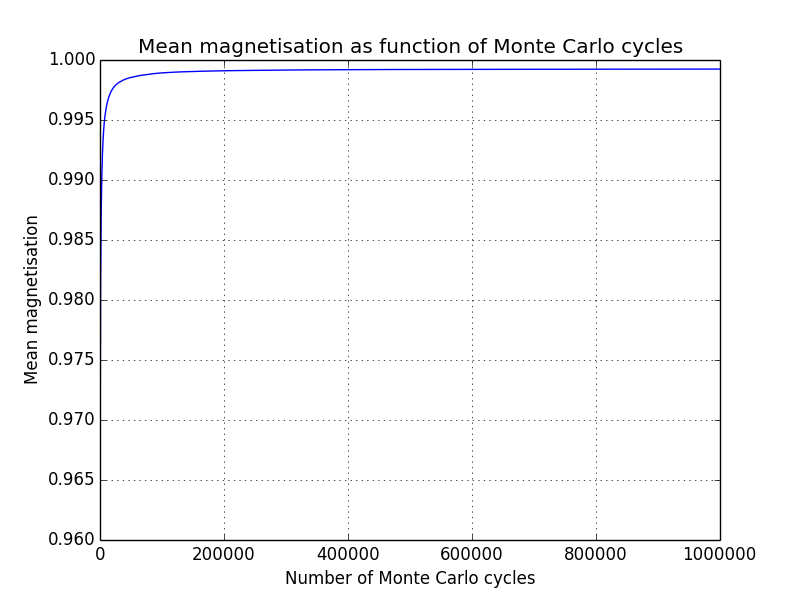
\includegraphics[height=1.7in]{4cmagnetisationrandom.png}
        \caption{Magnetization}
    \end{subfigure}%
    ~ 
    \begin{subfigure}[t]{0.6\textwidth}
        \centering
        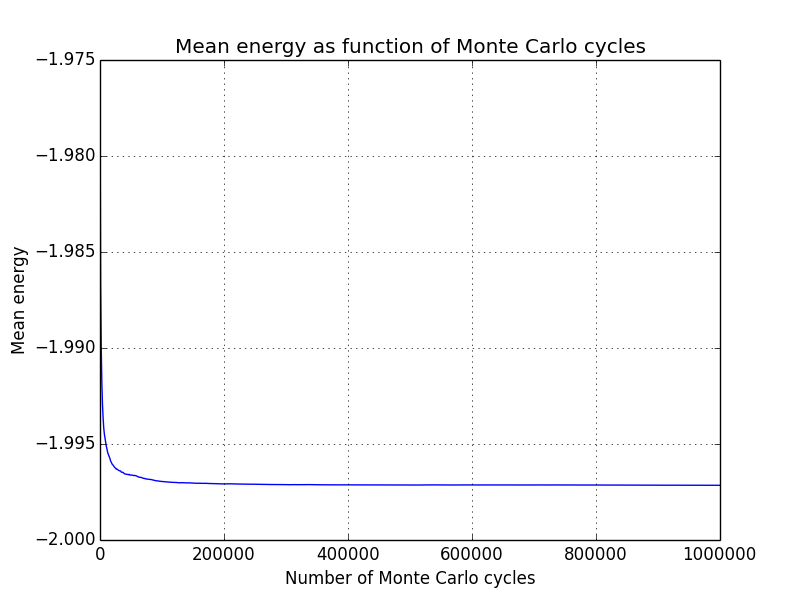
\includegraphics[height=1.7in]{4cenergyrandom.png}
        \caption{Energy}
    \end{subfigure}
    \caption{Plot of magnetization and energy as function of time corresponding to the number Monte Carlo cycles. Random spin orientation as start configuration and $T = 1.0$}
\end{figure*}

\begin{figure*}[t!]
    \centering
    \begin{subfigure}[t]{0.6\textwidth}
        \centering
        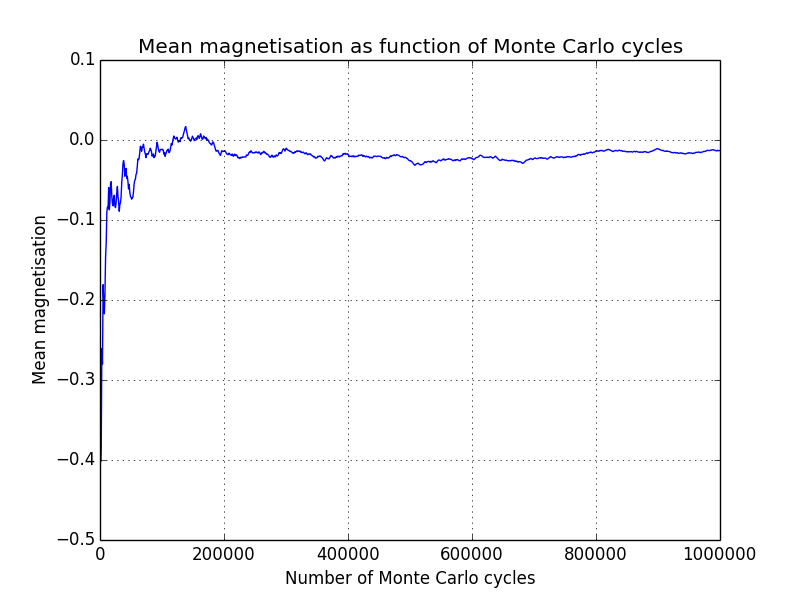
\includegraphics[height=1.7in]{4cmagnetisationrandom24.png}
        \caption{Magnetization}
    \end{subfigure}%
    ~ 
    \begin{subfigure}[t]{0.6\textwidth}
        \centering
        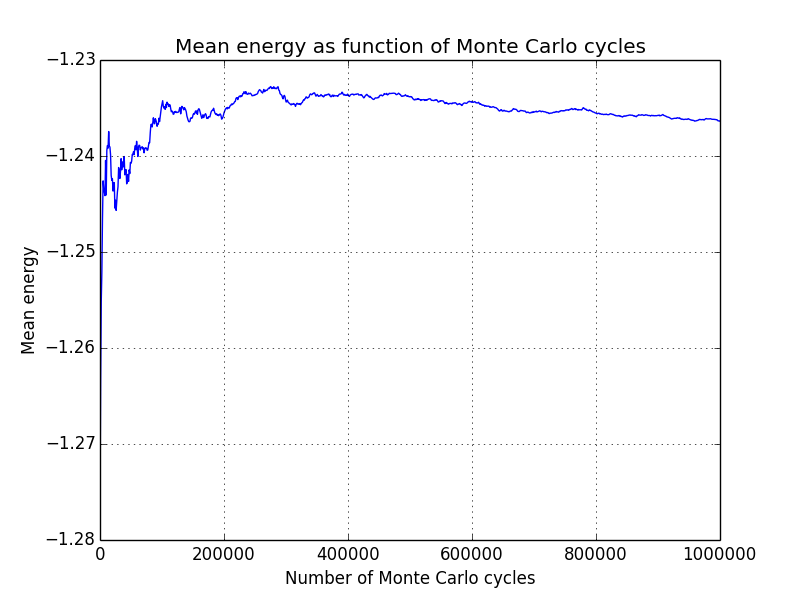
\includegraphics[height=1.7in]{4cenergyrandom24.png}
        \caption{Energy}
    \end{subfigure}
    \caption{Plot of magnetization and energy as function of time corresponding to the number Monte Carlo cycles.Random spin orientation as start configuration and $T = 2.4$}
\end{figure*}
\begin{figure*}[t!]
    \centering
    \begin{subfigure}[t]{0.6\textwidth}
        \centering
        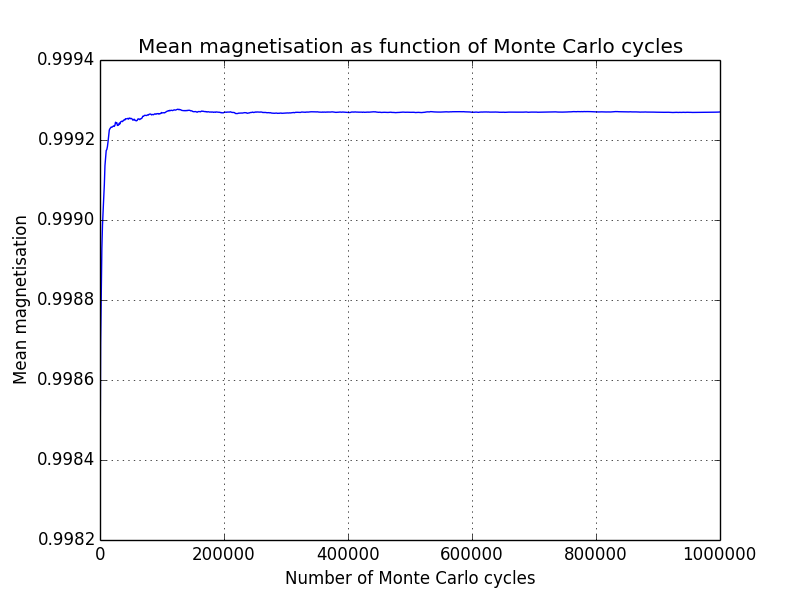
\includegraphics[height=1.7in]{4cmagnetisation.png}
        \caption{Magnetization}
    \end{subfigure}%
    ~ 
    \begin{subfigure}[t]{0.6\textwidth}
        \centering
        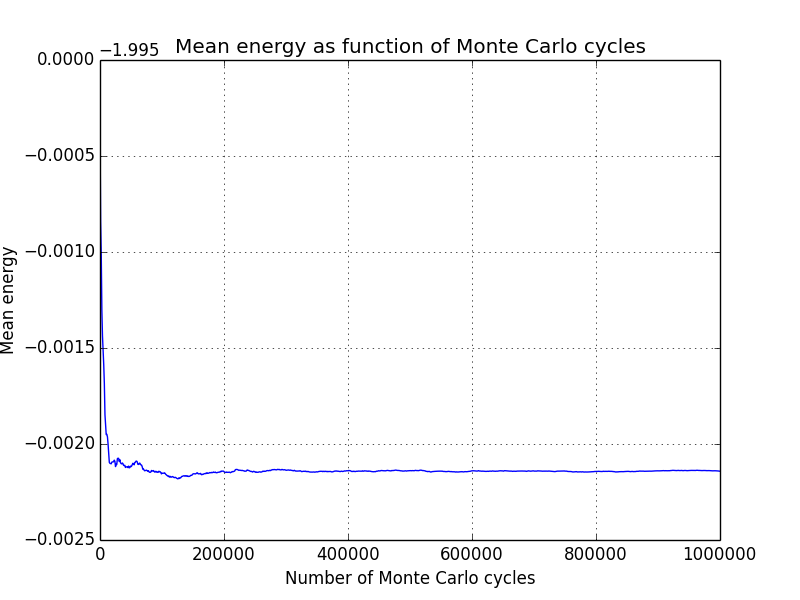
\includegraphics[height=1.7in]{4cenergy.png}
        \caption{Energy}
    \end{subfigure}
    \caption{Plot of magnetization and energy as function of time corresponding to the number Monte Carlo cycles. Ordered spin orientation as start configuration and $T = 1.0$}
\end{figure*}
\begin{figure*}[t!]
    \centering
    \begin{subfigure}[t]{0.6\textwidth}
        \centering
        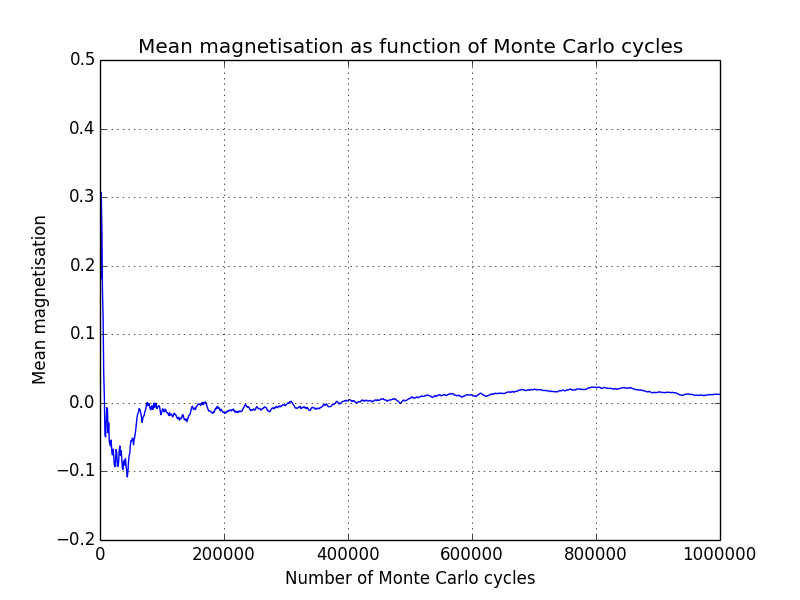
\includegraphics[height=1.7in]{4cmagnetisation24.png}
        \caption{Magnetization}
    \end{subfigure}%
    ~ 
    \begin{subfigure}[t]{0.6\textwidth}
        \centering
        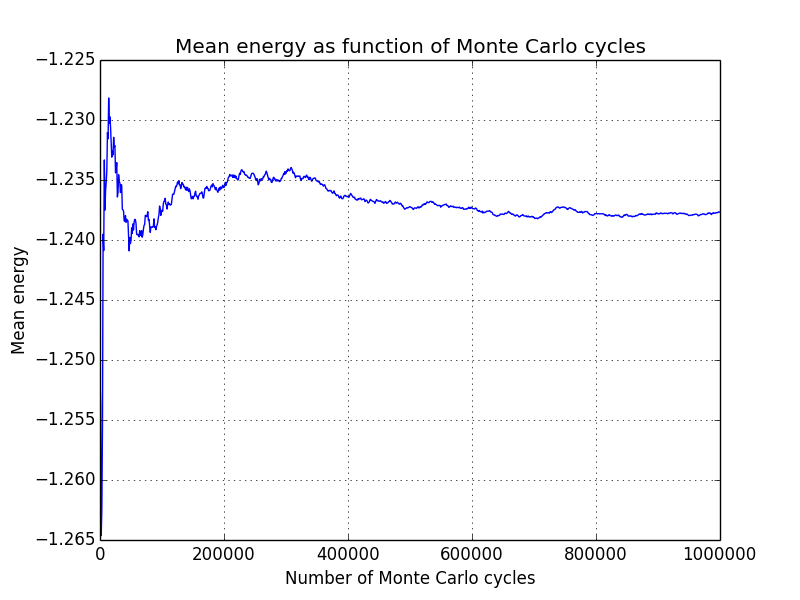
\includegraphics[height=1.7in]{4cenergy24.png}
        \caption{Energy}
    \end{subfigure}
    \caption{Plot of magnetization and energy as function of time corresponding to the number Monte Carlo cycles. Ordered spin orientation as start configuration and $T = 2.4$}
\end{figure*}

\begin{figure}[h]
\centering
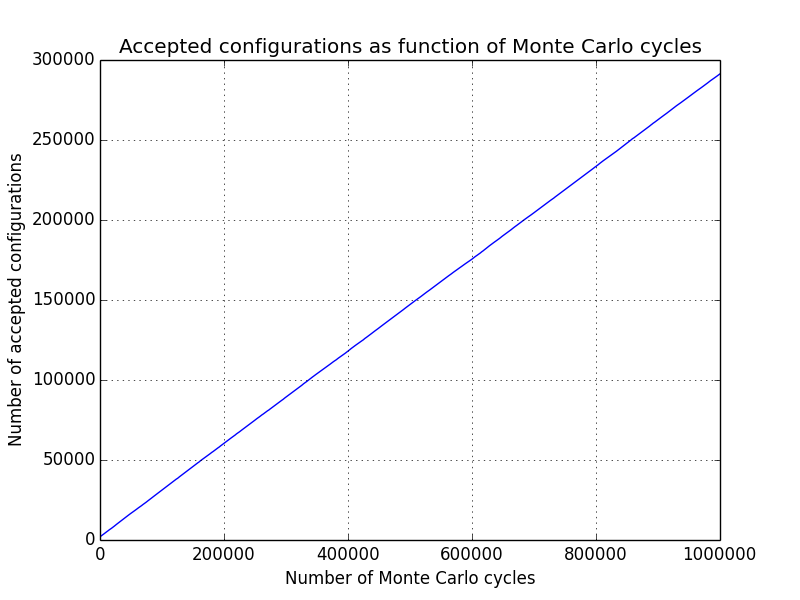
\includegraphics[width=0.6\textwidth]{4caccepted.png}
\caption{Total number of accepted configurations as function of the total number of Monte Carlo cycles.}
\end{figure}
\subsection*{Probability distribution}.
Now we want to look at the probability $P(E)$ for the previous system, with the same temperatures. In figure 
\begin{figure*}[t!]
    \centering
    \begin{subfigure}[t]{0.6\textwidth}
        \centering
        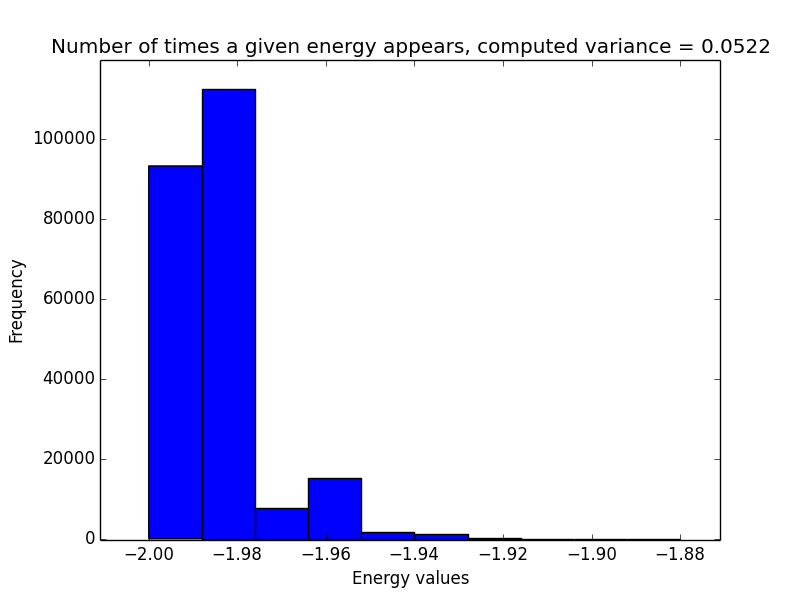
\includegraphics[height=1.7in]{4dT1.png}
        \caption{T = 1.0}
    \end{subfigure}%
    ~ 
    \begin{subfigure}[t]{0.6\textwidth}
        \centering
        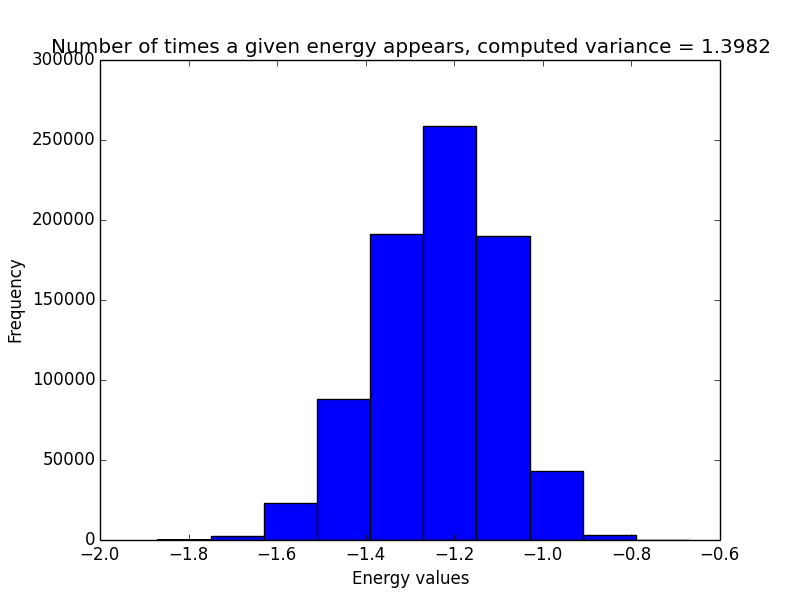
\includegraphics[height=1.7in]{4dT24.png}
        \caption{T = 2.4}
    \end{subfigure}
    \caption{Histogram with number of times a given energy appears in our computations after steady state has been reached. Computed variance is 1.3982 for T=2.4 and 0.0522 for T=1.0.}
\end{figure*}


\section*{Phase transition}
%4e) Figurer. Can you see an indication of a phase transition? 
\subsection*{Critical temperature}
%Estimate Tc. 
\subection*{Conclusion}
\subsection*{References}

\end{document}